\begin{center}
	\vspace{0.5cm}
	{\parbox{16cm}
		{\small{\centering{\textbf{Аннотация}\\
					\hspace{0.6cm} 
					В этом отчёте изложены результаты выполнения лабораторной работы «Виртуальный ЯМР». Предметом исследования в которой был спектр ЯМР, представленный в используемой программе "NMR" под номером $11$.
				}
			}
		}
	}
\end{center}

\textbf{\emph{Цель работы:}}
Решить обратную задачу ЯМР для представленного спектра, оценить относительную неоднородность постоянного магнитного поля.
\section{Теоретическое введение}
\subsection{Суть явления ЯМР}
Явление ЯМР заключается в резонансном поглощении электромагнитной энергии макроскопической системой ядерных магнитных моментов, помещенных в постоянное внешнее магнитное поле. Ядерные магнитные моменты связаны с наличием у протонов и нейтронов \textit{спинов}.

Энергия $E$ магнитного момента, находящегося в постоянном магнитном поле $\vec{B_0}$, равна
\begin{equation}
\label{E_in_field}
E = - (\vec{\mu}, \vec{B_0}) = -\mu B_0 \cos \theta = - g \beta_N B_0 m_z
\end{equation}
где $\theta$ -- угол между направлениями векторов $\mu$ и $B_0$, а $ m_z $ -- проекция спина на ось $z$, совпадающую с направлением $ B_0 $, $\beta_N = 5.0508 \cdot 10^{-27} \text{Дж}/\text{Тл}$ -- ядерный магнетон, $g$ -- так называемый фактор Ланде, представляющий из себя безразмерную величину (индивидуален для каждого вещества).
Протон имеет спин $ I = 1/2 $, поэтому возможные значения проекции спина на ось квантования равны $ m_z = \pm 1/2 $.

Из (\ref{E_in_field}) следует, что в магнитном поле $B_0$ происходит расщепление на два состояния, имеющие разную энергию.
Между этими уровнями возможны переходы при поглощении кванта электромагнитной энергии определенной частоты -- это и есть суть ЯМР.

Нам также потребуется связь между напряженностью постоянного магнитного поля $H_0$ и резонансной частотой $\nu_0$ поглощения переменного электромагнитного
поля: 

\begin{equation}
\label{eq2}
\nu_0 = \frac{\gamma}{2\pi}H_0
\end{equation}

где $\gamma$ -- это гиромагнитное отношение.

Среди параметров описывающих вид спектра одним из основных является химический сдвиг.
Привожу таблицу, которая потребуется нам для соотнесения полученных значений и уточнения структурной формулы исследуемого вещества:

\begin{figure}[h!]
	\centering
	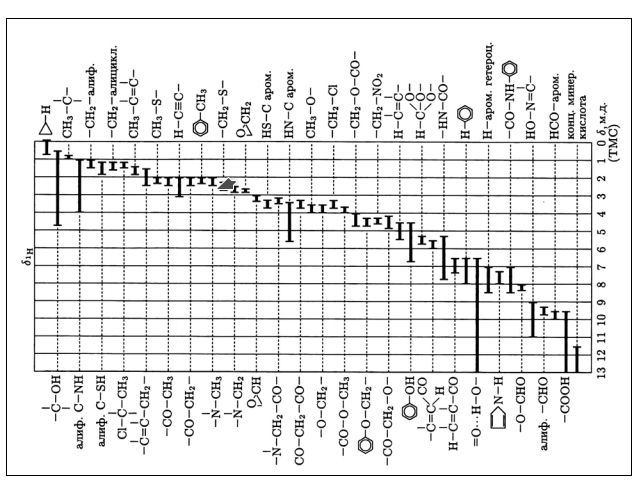
\includegraphics[width=0.55\linewidth]{tabl}
	\label{fig:tabl}
\end{figure}
